%\VignetteIndexEntry{North Carolina SIDS data set}
%\VignetteDepends{}
%\VignetteKeywords{spatial}
%\VignettePackage{spdep}
\documentclass[a4paper,10pt]{article} 
\usepackage{Sweave}
\usepackage{times}
\usepackage{mathptm}
\usepackage{hyperref}
\usepackage{natbib}

\setkeys{Gin}{width=0.95\textwidth}
\newcommand{\strong}[1]{{\normalfont\fontseries{b}\selectfont #1}}
\let\pkg=\strong
\RequirePackage{alltt}
\newenvironment{example}{\begin{alltt}}{\end{alltt}}
\newenvironment{smallexample}{\begin{alltt}\small}{\end{alltt}}
\newcommand{\code}[1]{\texttt{\small #1}}
\def\RR{\textsf{R}\/}
\def\SP{\texttt{S-PLUS}\/}
\def\SS{\texttt{S}\/}

\title{Introduction to the North Carolina SIDS data set} 
\author{Roger Bivand} 

\begin{document} 

\maketitle 




\section{Introduction}

This data set was presented first in \citet{symonsetal:1983}, analysed with
reference to the spatial nature of the data in \citet{cressie+read:1985},
expanded in \citet{cressie+chan:1989}, and used in detail in \citet{cressie:1991}. It is for
the 100 counties of North Carolina, and includes counts of numbers of
live births (also non-white live births) and numbers of sudden infant
deaths, for the 1974--1978 and 1979--1984 periods. In \citet{cressie+read:1985}, a listing of county neighbours based on shared boundaries
(contiguity) is given, and in \citet{cressie+chan:1989}, and in \citet[][pp. 386--389]{cressie:1991}, a different listing based on the criterion of
distance between county seats, with a cutoff at 30 miles. The county seat
location coordinates are given in miles in a local (unknown) coordinate
reference system. The data are also used to exemplify a range of functions
in the \SP~spatial statistics module user's manual \citep{kaluznyetal:1996}.


\section{Getting the data into \RR}

We will be using the \pkg{spdep} package, here version:
spdep, version 0.4-20, 2008-03-25, and the \pkg{maptools} package. The
data from the sources refered to above is collected in the
\code{nc.sids} data set in \pkg{spdep}. But to map it, we also
need access to data for the county boundaries for North Carolina;
this has been made available in the \pkg{maptools} package in
shapefile format\footnote{These data are taken with permission from:
\url{http://sal.agecon.uiuc.edu/datasets/sids.zip}.}. These data are known
to be geographical coordinates (longitude-latitude in decimal degrees)
and are assumed to use the NAD83 datum.

\begin{footnotesize}
\begin{Schunk}
\begin{Sinput}
> library(spdep)
\end{Sinput}
\end{Schunk}
\end{footnotesize}

The shapefile format presupposes that you have three files with extensions
\code{*.shp}, \code{*.shx}, and \code{*.dbf}, where the first contains the
geometry data, the second the spatial index, and the third the attribute
data. They are required to have the same name apart from the extension,
and are read using \code{read.shape()}. By default, this function reads
in the data in all three files, although it is only given the name of
the file with the geometry.
The imported object in \RR~has class \code{Map}, and is a list with
two components, \code{"Shapes"}, which is a list of shapes, and
\code{"att.data"}, which is a data frame with tabular data, one row
for each shape in \code{"Shapes"}. Here we will be using data previously read from the shapefile, and stored in the \code{nc.sids} data set:


\begin{footnotesize}
\begin{Schunk}
\begin{Sinput}
> data(nc.sids)
\end{Sinput}
\end{Schunk}
\begin{Schunk}
\begin{Sinput}
> plot(sidspolys, forcefill = FALSE)
> points(sidscents)
\end{Sinput}
\end{Schunk}
\end{footnotesize}
We can examine the names of the columns of the data frame to see what it
contains --- in fact some of the same columns that we will be examining
below, and some others which will be useful in cleaning the data
set. We will similarly convert the geometry format of the \code{Map}
object to that of a \code{polylist} object, which will be easier to
handle. Finally, we retreive the centroids of the county polygons to use
as label points. Using the \code{plot()} function for \code{"polylist"}
objects from \pkg{maptools}, we can display the polygon boundaries and
centroids, shown in Figure \ref{plotNC1}.

\begin{figure}[htbp]
\begin{center} 
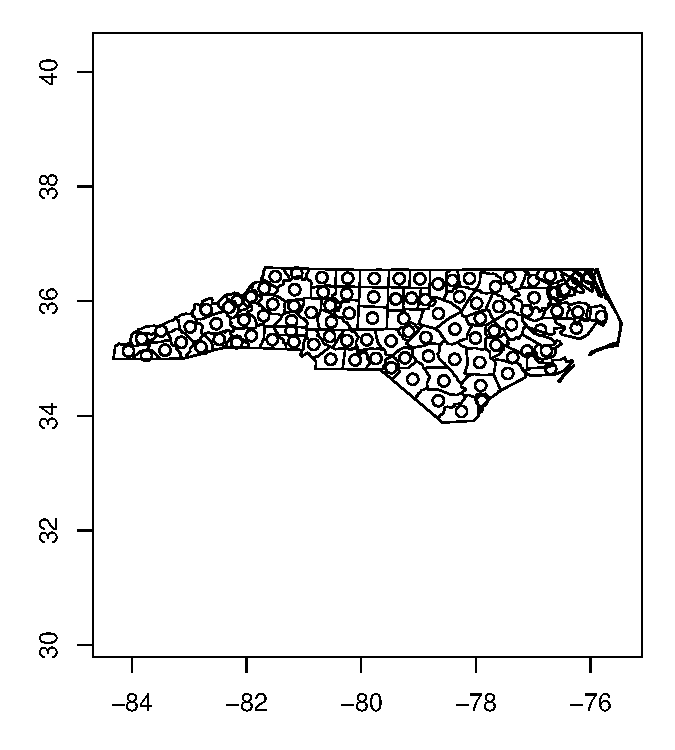
\includegraphics{Fig-bitmap-1.pdf}\end{center}
\caption{County boundaries and polygon centroids, North Carolina}
\label{plotNC1}
\end{figure}


It may be of interest to look at the structure of a polygon
list member. This is made up of a two-column matrix with polygon
coordinates. In general, each sub-polygon will have equal first
and last coordinates to ensure closure, but this is not absolutely
required. Rows in the coordinate matrix set to \code{NA} represent
breaks between sub-polygons, and are respected by the underlying
\RR~graphics functions. The attributes contain further information about
the polygon: \code{pstart} is a list with \code{from} and \code{to}
components, which are vectors of first and last rows in the matrix for
each sub-polygon in the object --- there are \code{nParts} elements
in both \code{from} and \code{to}. \code{RingDir} and \code{ringDir}
should be the same (but are not here, \code{ringDir} is correct, and
\code{RingDir} is wrong!), and are computed in two different ways to
determine whether each of the \code{nParts} sub-polygons runs clockwise
or counter-clockwise. Counter-clockwise sub-polygons are ``holes'' in
the surrounding sub-polygon. Finally, \code{bbox} contains the bounding
box of this object. Its appearance is shown in Figure \ref{poly6}.

\setkeys{Gin}{width=0.4\textwidth}
\begin{figure}[htbp]
\begin{center} 
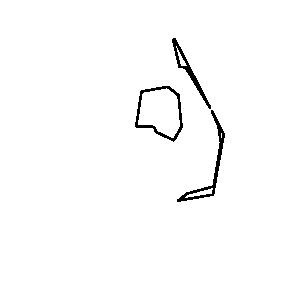
\includegraphics{sids-010}
\end{center}
\caption{Plot of polygon 56 from the list of polygons.}
\label{poly6}
\end{figure}
\setkeys{Gin}{width=0.95\textwidth}

\begin{footnotesize}
\begin{Schunk}
\begin{Sinput}
> round(t(sidspolys[[56]]), 3)
\end{Sinput}
\begin{Soutput}
        [,1]    [,2]    [,3]    [,4]    [,5]    [,6] [,7]    [,8]
[1,] -75.783 -75.773 -75.545 -75.703 -75.741 -75.783   NA -75.891
[2,]  36.225  36.229  35.788  36.050  36.050  36.225   NA  35.631
        [,9]   [,10]   [,11]   [,12]   [,13]   [,14]   [,15]   [,16]
[1,] -75.908 -76.021 -75.988 -75.818 -75.749 -75.729 -75.779 -75.891
[2,]  35.666  35.669  35.893  35.924  35.869  35.665  35.579  35.631
     [,17]   [,18]   [,19]   [,20]   [,21]   [,22]   [,23]   [,24]
[1,]    NA -75.491 -75.475 -75.521 -75.692 -75.749 -75.526 -75.457
[2,]    NA  35.670  35.564  35.281  35.235  35.190  35.228  35.617
       [,25]   [,26]
[1,] -75.534 -75.491
[2,]  35.769  35.670
attr(,"after")
[1] NA NA NA
attr(,"plotOrder")
[1] 1 2 3
attr(,"pstart")
attr(,"pstart")$from
[1]  1  8 18

attr(,"pstart")$to
[1]  6 16 26

attr(,"bbox")
[1] -76.02121  35.18983 -75.45698  36.22926
attr(,"RingDir")
[1] 1 1 1
attr(,"nParts")
[1] 3
attr(,"ringDir")
[1] 1 1 1
\end{Soutput}
\begin{Sinput}
> sidscents[56, ]
\end{Sinput}
\begin{Soutput}
[1] -75.80982  35.73548
\end{Soutput}
\end{Schunk}
\begin{Schunk}
\begin{Sinput}
> plot(sidspolys[[56]], type = "l", asp = 1, axes = FALSE, 
+     xlab = "", ylab = "")
\end{Sinput}
\end{Schunk}
\end{footnotesize}



We will now examine the data set reproduced from Cressie and collaborators,
included in \pkg{spdep}, and add the neighbour relationships used in
\citet{cressie+chan:1989} to the background map as a graph shown in Figure \ref{plot-CC89.nb}:

\begin{footnotesize}
\begin{Schunk}
\begin{Sinput}
> plot(sidspolys, border = "grey", forcefill = FALSE)
> plot(ncCC89.nb, sidscents, add = TRUE, col = "blue")
\end{Sinput}
\end{Schunk}
\end{footnotesize}

\begin{figure}[htbp]
\begin{center} 
\includegraphics{Fig-bitmap-2.pdf}\end{center}
\caption{Overplotting shapefile boundaries with 30 mile neighbour relations as a graph.}
\label{plot-CC89.nb}
\end{figure}

Printing the neighbour object shows that it is a neighbour list object, with a
very sparse structure --- if displayed as a matrix, only 3.94\% of cells
would be filled. Objects of class \code{nb} contain a list as long as
the number of counties; each component of the list is a vector with the
index numbers of the neighbours of the county in question, so that the
neighbours of the county with \code{region.id} of "1825" can be retreived
by matching against the indices. More information can be obtained by
using \code{summary()} on an \code{nb} object. Finally, we associate a
vector of names with the neighbour list, through the \code{row.names}
argument. The names should be unique, as with data frame row names.

\begin{footnotesize}
\begin{Schunk}
\begin{Sinput}
> ncCC89.nb
\end{Sinput}
\begin{Soutput}
Neighbour list object:
Number of regions: 100 
Number of nonzero links: 394 
Percentage nonzero weights: 3.94 
Average number of links: 3.94 
2 regions with no links:
2000 2099
\end{Soutput}
\begin{Sinput}
> r.id <- attr(ncCC89.nb, "region.id")
> ncCC89.nb[[match("1825", r.id)]]
\end{Sinput}
\begin{Soutput}
[1]  2 18 19
\end{Soutput}
\begin{Sinput}
> r.id[ncCC89.nb[[match("1825", r.id)]]]
\end{Sinput}
\begin{Soutput}
[1] 1827 1874 1880
\end{Soutput}
\end{Schunk}
\end{footnotesize}
The neighbour list object records neighbours by their order in
relation to the list itself, so the neighbours list for the county with
\code{region.id} "1825" are the second, eighteenth, and nineteenth in
the list. We can retreive their codes by looking them up
in the \code{region.id} attribute.

\begin{footnotesize}
\begin{Schunk}
\begin{Sinput}
> nc.sids[card(ncCC89.nb) == 0, ]
\end{Sinput}
\begin{Soutput}
     CNTY.ID BIR74 SID74 NWBIR74 BIR79 SID79 NWBIR79 east north
Dare    2000   521     0      43  1059     1      73  482   145
Hyde    2099   338     0     134   427     0     169  446   110
          x       y       lon      lat L.id M.id
Dare 439.65 3975.36 -75.66893 35.92070    2    4
Hyde 379.42 3920.72 -76.32823 35.42260    2    4
\end{Soutput}
\end{Schunk}
\end{footnotesize}
We should also note that this neighbour criterion generates two counties
with no neighbours, Dare and Hyde, whose county seats were more than
30 miles from their nearest neighbours. The \code{card()} function
returns the cardinality of the neighbour set. We need to return to
methods for handling no-neighbour objects later on. We will also show
how new neighbours lists may be constructed in \RR, and compare these
with those from the literature.


\subsection{Probability mapping}


Rather than review functions for measuring and modelling spatial
dependence in the \pkg{spdep} package, we will focus on probability
mapping for disease rates data. Typically, we have counts of the incidence
of some disease by spatial unit, associated with counts of populations
at risk. The task is then to try to establish whether any spatial units
seem to be characterised by higher or lower counts of cases than might
have been expected in general terms \citep{bailey+gatrell:1995}.

An early approach by \citet{choynowski:1959}, described by
\citet{cressie+read:1985} and \citet{bailey+gatrell:1995}, assumes,
given that the true rate for the spatial units is small, that as the
population at risk increases to infinity, the spatial unit case counts
are Poisson with mean value equal to the population at risk times the
rate for the study area as a whole. Choynowski's approach folds the two
tails of the measured probabilities together, so that small values, for
a chosen $\alpha$, occur for spatial units with either unusually high
or low rates. For this reason, the high and low counties are plotted
separately in Figure \ref{choymap}.

\begin{footnotesize}
\begin{Schunk}
\begin{Sinput}
> ch <- choynowski(nc.sids$SID74, nc.sids$BIR74)
\end{Sinput}
\end{Schunk}
\begin{Schunk}
\begin{Sinput}
> plot(sidspolys, forcefill = FALSE)
> legend(c(-84, -81), c(33.9, 34.5), fill = grey(c(2, 5)/7), 
+     legend = c("high", "low"), bty = "n", ncol = 2)
> plot(subset(sidspolys, ((ch$pmap < 0.05) & (ch$type))), 
+     col = grey(5/7), add = TRUE, forcefill = FALSE)
> plot(subset(sidspolys, ((ch$pmap < 0.05) & (!ch$type))), 
+     col = grey(2/7), add = TRUE, forcefill = FALSE)
\end{Sinput}
\end{Schunk}
\end{footnotesize}

\begin{figure}[htbp]
\begin{center} 
\includegraphics{Fig-bitmap-3.pdf}\end{center}
\caption{Probability map of North Carolina counties, SIDS cases 1974--78, $\alpha = 0.05$, reproducing \citet{cressie+read:1985}, Figure 1.}
\label{choymap}
\end{figure}


For more complicated thematic maps, it may be helpful to use ColorBrewer
(\url{http://colorbrewer.org}) colour palettes. Here we will only use
the grey sequential palette, available in \RR~in the \pkg{RColorBrewer}
package (the colours are copied here to avoid loading the package).

While the \code{choynowski()} function only provides the probability
map valyes required, the \code{probmap()} function returns raw (crude)
rates, expected counts (assuming a constant rate across the study area),
relative risks, and Poisson probability map values calculated using the
standard cumulative distribution function \code{ppois()}. This does not
fold the tails together, so that counties with lower observed counts
than expected, based on population size, have values in the lower tail,
and those with higher observed counts than expected have values in the
upper tail, as Figure \ref{poismap} shows.

\begin{footnotesize}
\begin{Schunk}
\begin{Sinput}
> pmap <- probmap(nc.sids$SID74, nc.sids$BIR74)
> brks <- c(0, 0.001, 0.01, 0.025, 0.05, 0.95, 0.975, 0.99, 
+     0.999, 1)
> cols <- c("#FFFFFF", "#F0F0F0", "#D9D9D9", "#BDBDBD", 
+     "#969696", "#737373", "#525252", "#252525", "#000000")
\end{Sinput}
\end{Schunk}
\begin{Schunk}
\begin{Sinput}
> plot(sidspolys, col = cols[findInterval(pmap$pmap, brks)], 
+     forcefill = FALSE)
> legend(c(-84, -81), c(33.9, 34.5), fill = cols, legend = leglabs(brks), 
+     bty = "n", ncol = 2)
\end{Sinput}
\end{Schunk}
\end{footnotesize}

\begin{figure}[htbp]
\begin{center} 
\includegraphics{Fig-bitmap-4.pdf}\end{center}
\caption{Probability map of North Carolina counties, SIDS cases 1974--78, reproducing \citet{kaluznyetal:1996}, p. 57, Figure 3.28.}
\label{poismap}
\end{figure}

Marilia Carvalho (personal communication) and Virgilio G�mez Rubio
\citep{gomez-rubio+ferrandiz+lopez:2003} have pointed to the unusual
shape of the distribution of the Poisson probability values (Figure
\ref{poishist}), repeating the doubts about probability mapping voiced
by \citet[][p. 392]{cressie:1991}: ``an extreme value $\ldots$ may be
more due to its lack of fit to the Poisson model than to its deviation
from the constant rate assumption''. There are many more high values
than one would have expected, suggesting perhaps overdispersion, that
is that the ratio of the mean and variance is larger than unity.


\begin{footnotesize}
\begin{Schunk}
\begin{Sinput}
> hist(pmap$pmap, main = "")
\end{Sinput}
\end{Schunk}
\end{footnotesize}


\begin{figure}[htbp]
\begin{center} 
\includegraphics{Fig-bitmap-5.pdf}\end{center}
\caption{Histogram of Poisson probability values.}
\label{poishist}
\end{figure}


One ad-hoc way to assess the impact of the possible failure of our
assumption that the counts follow the Poisson distribution is to estimate
the dispersion by fitting a general linear model of the observed counts
including only the intercept (null model) and offset by the observed
population at risk (suggested by Marilia Carvalho and associates):

\begin{footnotesize}
\begin{Schunk}
\begin{Sinput}
> res <- glm(nc.sids$SID74 ~ offset(log(BIR74)), data = nc.sids, 
+     family = "quasipoisson")
> stdres <- rstandard(res)
> brks <- c(-Inf, -2, -1.5, -1, 1, 1.5, 2, +Inf)
> cols <- c("#F7F7F7", "#D9D9D9", "#BDBDBD", "#969696", 
+     "#737373", "#525252", "#252525")
\end{Sinput}
\end{Schunk}
\begin{Schunk}
\begin{Sinput}
> plot(sidspolys, col = cols[findInterval(stdres, brks)], 
+     forcefill = FALSE)
> legend(c(-84, -81), c(33.9, 34.5), fill = cols, legend = leglabs(brks), 
+     bty = "n", ncol = 2)
\end{Sinput}
\end{Schunk}
\end{footnotesize}

The dispersion is equal to 2.2786, 
much greater than unity; we calculate the corrected
probability map values by taking the standardised residuals of the
model, taking the size of the dispersion into account; the results
are shown in Figure \ref{poismap2}. Many fewer counties appear
now to have unexpectedly large or small numbers of cases. This is
an ad-hoc adjustment made because \RR~provides access to a wide
range of model-fitting functions that can be used to help check our
assumptions. \citet{gomez-rubio+ferrandiz+lopez:2003} chose rather to
construct a probability map under the hypothesis that data are drawn
from a Negative Binomial.

\begin{figure}[htbp]
\begin{center} 
\includegraphics{Fig-bitmap-6.pdf}\end{center}
\caption{Standardised residual values from the fit of a quasi-Poisson fit of the null model for SIDS rates 1974-78, North Carolina counties.}
\label{poismap2}
\end{figure}



So far, none of the maps presented have made use of the spatial
dependence possibly present in the data. A further elementary step that
can be taken is to map Empirical Bayes estimates of the rates, which
are smoothed in relation to the raw rates. The underlying question
here is linked to the larger variance associated with rate estimates
for counties with small populations at risk compared with counties with
large populations at risk. Empirical Bayes estimates place more credence
on the raw rates of counties with large populations at risk, and modify
them much less than they modify rates for small counties. In the case
of small populations at risk, more confidence is placed in either the
global rate for the study area as a whole, or for local Empirical Bayes
estimates, in rates for a larger moving window including the neighbours of
the county being estimated. The function used for this in \pkg{spdep} is
\code{EBlocal()}, initially contributed by Marilia Carvalho. It parallels
a similar function in GeoDa, but uses the \citet{bailey+gatrell:1995}
interpretation of \citet{marshall:1991}, rather than that in GeoDa
\citep{anselin+syabri+smirnov:2002}.

\begin{footnotesize}
\begin{Schunk}
\begin{Sinput}
> res <- EBlocal(nc.sids$SID74, nc.sids$BIR74, ncCC89.nb, 
+     zero.policy = TRUE)
> brks <- c(-Inf, 2, 2.5, 3, 3.5, Inf)
> cols <- c("#F7F7F7", "#CCCCCC", "#969696", "#636363", 
+     "#252525")
> sub <- is.finite(res$est)
\end{Sinput}
\end{Schunk}
\begin{Schunk}
\begin{Sinput}
> plot(sidspolys, forcefill = FALSE)
> legend(c(-84, -81), c(33.9, 34.5), fill = cols, legend = leglabs(brks), 
+     bty = "n", ncol = 2)
> plot(subset(sidspolys, sub), col = cols[findInterval(res$est[sub] * 
+     1000, brks)], add = TRUE, forcefill = FALSE)
> points(sidscents[!sub, ], pch = 8)
\end{Sinput}
\end{Schunk}
\end{footnotesize}

The results are shown in Figure \ref{EBlocal}. Like other relevant
functions in \pkg{spdep}, \code{EBlocal()} takes a \code{zero.policy}
argument to allow missing values to be passed through. In this case,
no local estimate is available for the two counties with no neighbours,
marked by stars.

\begin{figure}[htbp]
\begin{center} 
\includegraphics{Fig-bitmap-7.pdf}\end{center}
\caption{Local Empirical Bayes estimates for SIDS rates per 1000 using the 30 mile county seat neighbours list.}
\label{EBlocal}
\end{figure}


\section{Preliminary exploration of the data (incomplete)}

One of the first steps taken by \citet{cressie+read:1985} is to try to
bring out spatial trends by dividing North Carolina up into $4\times4$
rough rectangles. Just to see how this works, let us map these rough
rectangles before proceeding further (see Figure \ref{LMmap}). We need
to recall that the \code{nc.sids} data frame is not in the same order
as the polygons.


\begin{footnotesize}
\begin{Schunk}
\begin{Sinput}
> both <- factor(paste(nc.sids$L.id, nc.sids$M.id, sep = ":"))
> cols <- sample(rainbow(length(table(unclass(both)))))
\end{Sinput}
\end{Schunk}
\begin{Schunk}
\begin{Sinput}
> plot(sidspolys, col = cols[both[order(nc.sids$CNTY.ID)]], 
+     forcefill = FALSE)
> legend(c(-84, -81), c(33.5, 34.6), legend = levels(both), 
+     fill = cols, bty = "n", cex = 0.9, y.intersp = 0.9, 
+     ncol = 2)
\end{Sinput}
\end{Schunk}
\end{footnotesize}

\begin{figure}[htbp]
\begin{center} 
\includegraphics{Fig-bitmap-8.pdf}\end{center}
\caption{Rough rectangles used by \citet{cressie+read:1985} to bring out spatial trends.}
\label{LMmap}
\end{figure}

(document to be extended in next release --- terminates here to at least show how \pkg{maptools} and \pkg{spdep} can be used together).


\section*{References}

\begin{description}

\bibitem[\protect\citeauthoryear{Anselin, Syabri and Smirnov}{Anselin, Syabri and Smirnov}{2002}]{anselin+syabri+smirnov:2002}
Anselin, L., Syabri, I., Smirnov, O., 2002.
\newblock {Visualizing Multivariate Spatial Correlation with Dynamically Linked Windows}.
\newblock {In Anselin, L., Rey, S. (Eds.), Proceedings, CSISS Workshop on New Tools for Spatial Data Analysis, Santa Barbara, CA, May 10-11, 2002. Center for Spatially Integrated Social Science},
\newblock 20 pp., {\url{http://sal.agecon.uiuc.edu/csiss/pdf/multilisa.pdf}}.

\bibitem[\protect\citeauthoryear{Bailey and Gatrell}{Bailey and Gatrell}{1995}]{bailey+gatrell:1995}
Bailey, T.~C., Gatrell, A.~C., 1995.
\newblock {Interactive Spatial Data Analysis}.
\newblock {Harlow: Longman},
\newblock 413 pp.

\bibitem[\protect\citeauthoryear{Choynowski}{Choynowski}{1959}]{choynowski:1959}
Choynowski, M., 1959
\newblock {Maps based on probabilities}.
\newblock {Journal of the American Statistical Association},
\newblock 54 (286), {385--388}.

\bibitem[\protect\citeauthoryear{Cressie}{Cressie}{1991}]{cressie:1991}
Cressie, N., 1991.
\newblock {Statistics for spatial data}.
\newblock {New York: Wiley},
\newblock 900 pp.

\bibitem[\protect\citeauthoryear{Cressie and Chan}{Cressie and Chan}{1989}]{cressie+chan:1989}
Cressie, N., Chan N.~H., 1989.
\newblock {Spatial modelling of regional variables}.
\newblock {Journal of the American Statistical Association},
\newblock 84 (406), {393--401}.

\bibitem[\protect\citeauthoryear{Cressie and Read}{Cressie and Read}{1985}]{cressie+read:1985}
Cressie, N., Read, T.~R.~C., 1985.
\newblock {Do sudden infant deaths come in clusters?}.
\newblock {Statistics and Decisions},
\newblock {Supplement Issue 2, 333--349}.

\bibitem[\protect\citeauthoryear{Cressie and Read}{Cressie and Read}{1989}]{cressie+read:1989}
Cressie, N., Read, T.~R.~C., 1989.
\newblock {Spatial data-analysis of regional counts}.
\newblock {Biometrical Journal},
\newblock 31 (6), {699--719}.

\bibitem[\protect\citeauthoryear{G�mez Rubio, Ferr�ndiz and L�pez}{G�mez Rubio, Ferr�ndiz and L�pez}{2003}]{gomez-rubio+ferrandiz+lopez:2003}
G�mez Rubio, V., Ferr�ndiz, J., L�pez, A., 2003
\newblock {Detecting Disease Clusters with \RR}.
\newblock {In: Hornik, K., Leisch, F., Zeilis, A. (Eds), Proceedings of the 3rd International Workshop on Distributed Statistical Computing, Vienna, Austria},
\newblock 15 pp., {(\url{http://www.ci.tuwien.ac.at/Conferences/DSC-2003/Proceedings/GomezRubioEtAl.pdf})}.

\bibitem[\protect\citeauthoryear{Kaluzny et al.}{Kaluzny et al.}{1996}]{kaluznyetal:1996}
Kaluzny, S.~P., Vega, S.~C., Cardoso, T.~P., Shelly, A.~A., 1996.
\newblock {\SP~SPATIALSTATS user's manual version 1.0}.
\newblock {Seattle: MathSoft Inc.},
\newblock 226 pp.

\bibitem[\protect\citeauthoryear{Marshall}{Marshall}{1991}]{marshall:1991}
Marshall, R.~M., 1991.
\newblock {Mapping disease and mortality rates using Empirical Bayes Estimators}.
\newblock {Applied Statistics},
\newblock 40 (2), {283--294}.

\bibitem[\protect\citeauthoryear{Symons et al.}{Symons et al.}{1983}]{symonsetal:1983}
Symons, M.~J., Grimson, R.~C., Yuan, Y.~C., 1983.
\newblock {Clustering of rare events}.
\newblock {Biometrics},
\newblock 39 (1), {193--205}.

\end{description}

\end{document}

